\documentclass[12pt]{article}

\usepackage[english]{babel}
\usepackage{listings}
\usepackage{graphicx}

\setlength\textwidth{7in} 
\setlength\textheight{9.5in} 
\setlength\oddsidemargin{-0.25in} 
\setlength\topmargin{-0.25in} 
\setlength\headheight{0in} 
\setlength\headsep{0in} 
\sloppy 

 
\begin{document}
\title{Strongly Connected Components}
\author{Thomas Schreiber}
\maketitle



\begin{abstract}
In computer science the graph data structure can be employed to solve a large set of problems. One task that is often needed is to find the \emph{strongly connected components} of a given graph. This paper explores Kosaraju's algorithm, a testing suite that benchmarks the performance of a strongly connected component algorithm in \emph{Python}, and reflects on the challenges and lessons that were taken from the authors experience.
\end{abstract}


\section{Finding Strongly Connected Components}

\ \ \ \ Computer scientists find extremely interesting ways to represent information in abstract ways. Problems can be more efficiently solved by breaking them into smaller pieces. Dates of the year can be entries in a table. Varying values can be stored in a heap structure for quick retrieval of the minimum or maximum value. Locations around the world can be represented as vertices with paths connecting each city to the next.

\begin{figure}[h!]
  \centering
  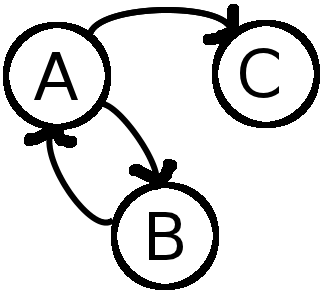
\includegraphics[width=0.25\textwidth]{simplegraph.png}
    \caption{A simple directed graph.}
\end{figure}

Graphs can represent very complex structures due to the amount of information they can represent. Throughout a graph each vertex contains data about how it relates or connects to other vertices. Due to this and other features graphs can be used in surprising ways. From molecular molecules to state-space models used in NASA's flight controls\cite{NASA} graphs are used to model everything from the atomic to the galactic scale.

One task that is often needed when dealing with graphs is to find the strongly connected components of a graph. A strongly connected component is a subgraph, $ G_s $, of the original graph, $ G $, wherein a path exists from any vertex $ v \in G_s$ to any other vertex $ u \in G_s$. Indeed finding the strongly connected components of a graph is used by NASA to simplify state-space models quickly\cite{NASA}. The remainder of this paper explores one popular algorithm for identifying the strongly connected components of a given graph.

  \subsection{Kosaraju's algorithm}
\ \ \ \ Created in 1978 by Rao S. Kosaraju, Kosaraju's algorithm may not necissarily be the most effecient algorithm for finding strongly connected components, but is widely published and easy to explain. In fact the entire algorithm can be written as a four step process\cite{CLRS}\cite{Narahari}.

    \begin{enumerate}
      \item Perform a depth-first-search on the graph keeping track of the finish times of each vertex.
      \item Compute the transpose of the graph.
      \item Perform a depth-first-search on the transposed graph in reverse order of the first DFS finish times.
      \item Output the vertices of each tree in the depth-first forest formed in step 3.
    \end{enumerate}

\begin{figure}[h!]
  \centering
  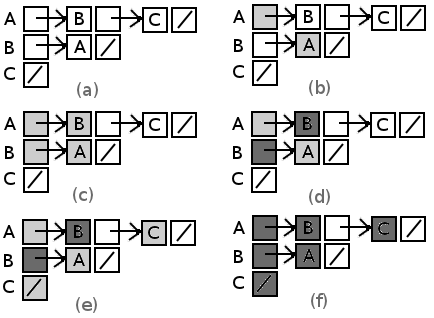
\includegraphics[width=0.5\textwidth]{dfsadjacencylist.png}
    \caption{A depth-first-search performed on an adjacency list.}
\end{figure}

Performing a depth-first-sort is an involved process. Take the simple graph in \emph{figure 1}, and it's adjacency list representation in \emph{figure 2a}. Starting with vertex 'A' we color it \emph{undiscovered} (\emph{figure2b}), and begin traversing the adjacency list of the vertices connected to 'A'. We then come to vertex 'B' which we recusively \emph{visit} (\emph{figure 2c}). Now, we can visit the \emph{undiscovered} vertices adjacent to 'B', but there are no undiscovered vertices adjacent to 'B' so we color it \emph{visited} (\emph{figure 2d}). This returns us to our traversal of 'A's adjacent vertices of which we now visit 'C' (\emph{figure 2e}). Finally, with 'C' visited all of 'A's adjacent nodes are visited. So, 'A' is colored visited (\emph{figure 2f}).

Once the graph has been transposed we can repeat the above process in reverse order of the recorded finish times for each vertex. In the example graph, \emph{figure 1 and 2}, the last finish time was vertex 'A'. Performing the DFS on the transposed graph starting with 'A' will tell us that 'A' and 'B' are part of the same tree in the depth-first forest and thus a strongly connected component. Leaving only 'C' which is a stronly connected component consisting only of itself. 

  \subsection{Time Complexity}
\ \ \ \ In order to compute Kosaraju's algorithm a number of specific things must occur. Given a graph, $ G(V,E) $, each vertex $v \in V$ must be initialized to an undiscovered state. Next, a DFS is performed requiring each edge $e \in E$ to be traversed. Then, to compute the transpose of G, $ G^T $, every vertex and edge of G must be processed. We perform another DFS on $ G^T $ taking additional time. Outputing the result takes S operations, where $ S \le V$. If we let all of the constant time operations equal C we have an algorithm of time complexit:

\[
\theta(|V| + |E| + |V| + |E| + |E| + S + C) = \theta(3|E| + 3|V| + C) = \theta(|V| + |E|)
\]

So, Kosaraju's algorithm has a time complexity of $ \theta(|V| + |E|) $. There exist other algorithms, such as Tarjan's algorithm, that have a time complexity of $ \theta(|V| lg |V|) $ \cite{Narahari}. However, the experimentation focused on Kosaraju's algorithm

\section{Experimentation}

\ \ \ \ The objective of the experiment was to test Kosaraju's algorithm on a variety of randomly generated graphs. The algorithm was implemented in \emph{Python}, and the experimentation was conducted on an Intel(R) Core(TM)2 Duo 2.26GHz workstation with 4GB RAM under Debian Linux 6.0. Due to the way in which the Python module 'os' handles clock timing under Linux the results did not have enough resolution to accurately record the time intervals for each use of the algorithm. Instead the \emph{time.time()} function was used which returns the actual time in epoch form. In order to account for other processes causing error in the start and finish times thousands of data points were collected for each random graph generation algorithm. 

Graphs were created using Python's built-in data structures. Each graph was represented by a dictionary whose keys were vertices. The values that these keys were paired with contained the current state of the vertex in a DFS (\emph{ie.} "undiscovered", "discovered", or "unvisited") and a list of the vertices that were adjacent to the current vertex. Care had to be taken in order to ensure that operations in Python (such as list append) happened in constant time.

  \subsection{Verifying the implementations correctness}
  \ \ \ \ The correctness of the implementation needed to be confirmed before the testing was to begin. This posed an interesting problem, because predicting the number of strongly connected components in a randomly generated graph can be very difficult. A unique algorithm for generating graphs was written in order to automate testing.
  
  The algorithm creates a set of disjoint \emph{cliques}, graphs that are completely connected, and randomly adds edges connecting the cliques ensuring that no cycle is ever formed between any two cliques (\emph{appendix 1}).
  
  The clique algorithm was used to generate 100 graphs of varying sizes, and processed by Kosaraju's algorithm. This process was repeated 10 times, and each one gave valid output. The results of one of the tests can be seen in \emph{figure 3}.
  
  With these results and a number of handmade tests designed to try and fuzz out bugs it was concluded that the implementation of Kosaraju's algorithm was correct enough that on large test data the result would be indicative of the algorithms actual time complexity. 

\begin{figure}[h!]
    \centering
      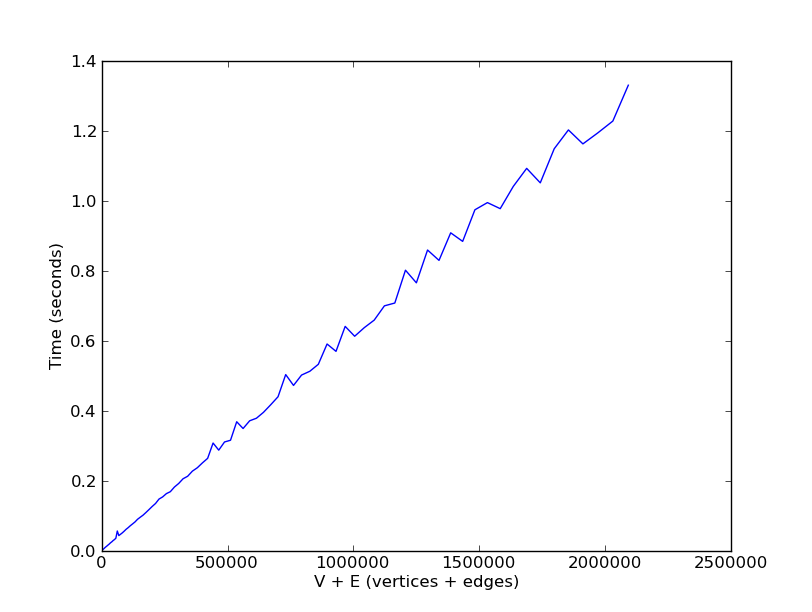
\includegraphics[width=0.6\textwidth]{cliquesForTesting.png}
        \caption{Testing of Kosaraju's algorithm with clique forests}
\end{figure} 

  \subsection{Random graphs with a specific number of edges}
  \ \ \ \ The first random graph that was attempted for experimentation attempted to maximize the randomness (\emph{appendix 2}). Given the number of vertices and the number of edges this algorithm picked any edge from the set of possible edges and added it to the graph. After some careful consideration parallel edges were forbidden, because they made the graphs less interesting for this experiments purposes.
  
  The results of this test went mostly as planned. In \emph{figure 4} we see that excepting for about 10 of the 1,000 data points the algorithm indeed does follow a linear asymptotic behavior as its $ \theta(|V| + |E|) $ time complexity predicts.
  
  \begin{figure}[h!]
    \centering
      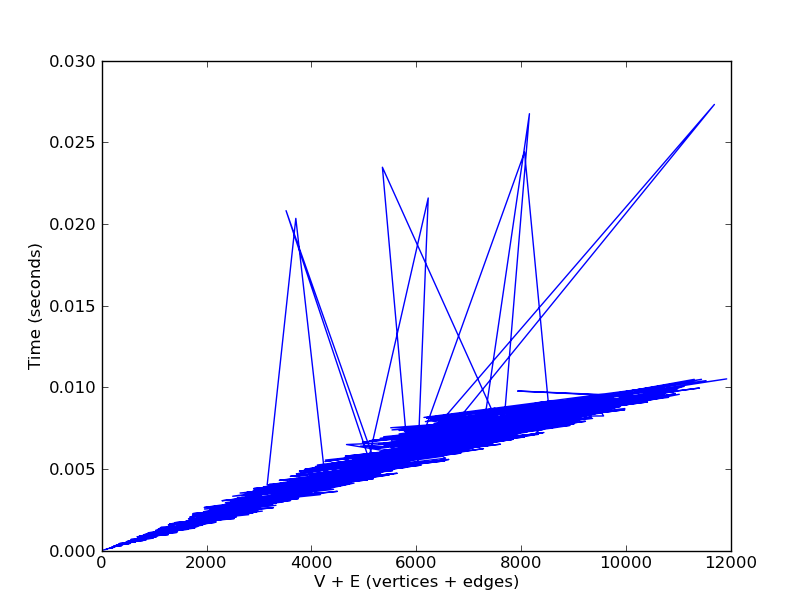
\includegraphics[width=0.6\textwidth]{GibsondirectedGraph.png}
        \caption{Running times and graph sizes generated by randGraph1}
\end{figure} 

  The ten data points that are wildly out of proportion of the other data points could be cause from other processes on the system used interfering with the test, artifacts of strange behavior inside the python interpreter, or bugs in the implementation. 
  
  \subsection{Random graphs with known vertex out-degree}
  \ \ \ \ The results from the first random graph generation algorithm were promising, but there were some improvements that could be made. For one, if only a few vertices end up with most of the edges the resulting graph have no strongly connected components containing more than a single vertex. Also, while it is unlikely it is possible that the first random graph generation could enter an infinite loop if parallel edges are repeatedly generated.
  
  To confront these issues a second random graph generation algorithm was written (\emph{appendix 3}). This algorithm allowed the max out-degree for all of the vertices to be controlled. The python random module was also utilized to take samples of all possible edges and add the sample to the adjacency list of the current vertex.
  
    \begin{figure}[h!]
    \centering
      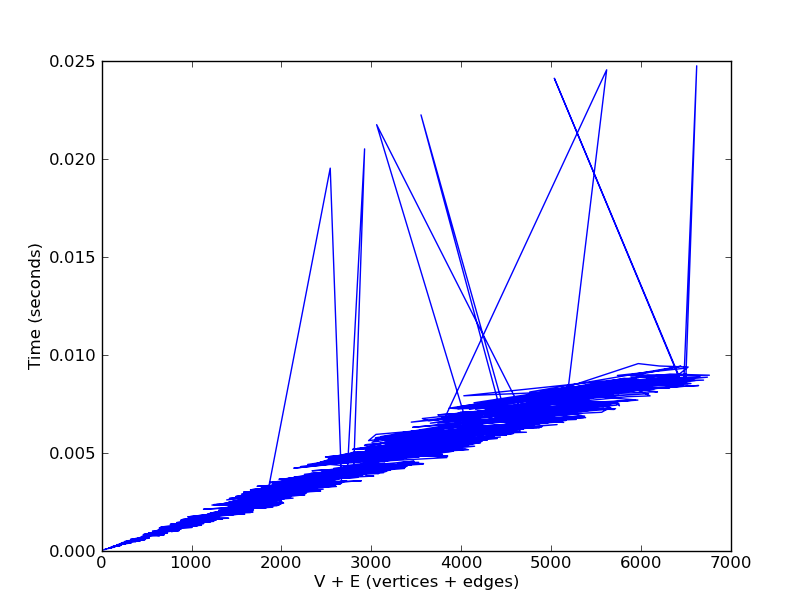
\includegraphics[width=0.6\textwidth]{Graphoutmax3.png}
        \caption{Running times and graph sizes where the out-degree of all vertices was limited to 3}
\end{figure} 

  For the experiment the maximum out-degree was limited to three. Again the strongly connected components algorithm was run on an input of 1000 graphs this time generated by the new algorithm (\emph{figure 5}). The results are similar to those found in section 2.2.  Again, about 10 data points seem to be wildly out of proportion, but the other 99.9\% of the data is in line with our expectations.
  
  \subsection{Random undirected graphs}
  \ \ \ \ At this point the results were very promising. Still, upon visual inspection of the graphs that were generated from the two previous algorithms a common pattern emerged. Depending on the number of edges in the graph there would either be no strongly connected components with more than two vertices, or the resultant graph would have one large connected component with all of the rest of the vertices in strongly connected components containing just the one vertex.
  
  The solution to this problem was to create yet another random graph generation algorithm that creates an undirected graph (\emph{appendix 4}). This algorithm works in much the same way as the one in section 2.2. The only difference is now for every pair of vertices $ v,u \in V $ of graph $ G $ that are randomly chosen edges $ (v,u) $ and $ (u,v) $ are added to the graph.
  
  This last of the random graph generation algorithms was used to produce an additional 1,000 graphs of size ranging from 2 to 1,000 vertices. Again, the results are as expected. Apart from a very small amount results that seem to be in error the result follow a nice linear path (\emph{figure 6}). 
  
     \begin{figure}[h!]
    \centering
      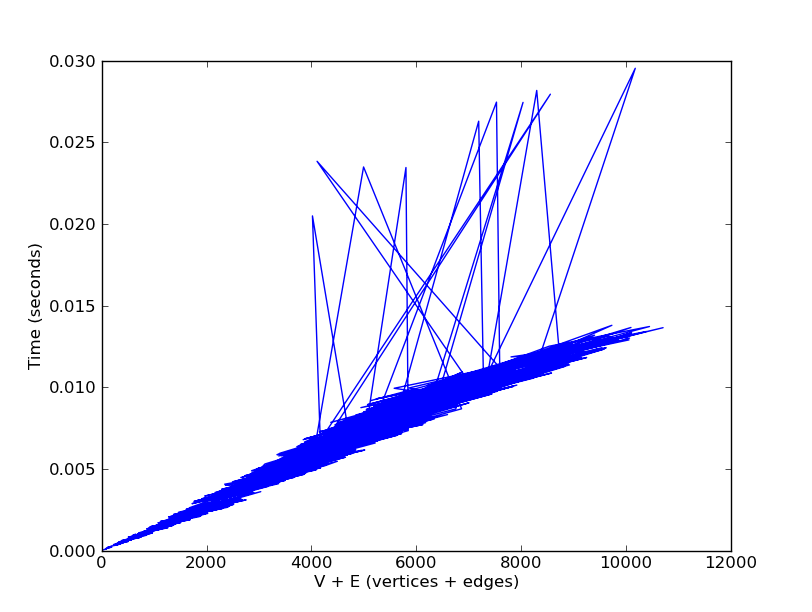
\includegraphics[width=0.6\textwidth]{undirectedGraph.png}
        \caption{Running times and graph sizes of undirected graphs}
\end{figure} 

  \subsection{Experimental results}
  \ \ \ \ With approximately 4,000 data points collected, from a range of different styles of graphs with wide range in the number of vertices and edges, a definitive trend can be seen. Accounting for about 0.01\% error there is a direct linear relationship with the number of vertices plus the number of edges and the running time of out implementation of Kosaraju's algorithm. 

\section{Reflections}

  \ \ \ \ Perhaps the most suprising aspect of this experiment was finding how diverse a random graph generation could be. While four specific graph generation algorithms were used it seems there are quite a number of things to consider with random graphs. The amount of time allotted for this project only allowed for a brief introduction to this very interesting topic, but I hope to take a deeper look into the subject in the future.
  
  The strange anomoulous behaviour that happened in about 0.01\% of the tests is also interesting. Finding the cause of these strange results proved to be extremely hard in Python. If I were to repeat this experiment in the future I would use a lower level language such as C and in general try to maximize control over the operation of the algorithm. This would help identify why a very small subset of the data took nearly twice the amount of time as the algorithm predicts.
  
  Using Python did have its advantages as well. This was the first time that I have gotten hands on experience with the matplotlib. For some time I have wanted experience with a library that visually represents large amounts of data. I found matplotlib easy to use, and it did a wonderfull job of creating cartesian graphs for this report.

\section{Conclusion}

\ \ \ \ Graphs are used to represent many things in our lives today. From molecules to transportation graphs help us model the world around us. In this paper we have taken an in depth look at one common task associated with graphs. Kosaraju's algorithm was implemented and tested. In oder to verify the time complexity of the implementation a large number of tests were run on various randomly generated graphs. The results were as expected, but the experience of conducting the experiment was suprisingly enlightening.

\

\

\begin{thebibliography}{9}


\bibitem{CLRS} Cormen, Thomas H.. \emph{Introduction to algorithms } .  Cambridge, Mass.: MIT Press, 2001. Print. pp. 524--560.

\bibitem{Hein}
Hein, James L.. \emph{Discrete structures, logic, and computability  .} 3rd ed. Sudbury: Jones and Bartlett, 2010. Print. pp. 56--64.

\bibitem{Narahari}
Narahari, Y.. "7.5.3 Strong Components." \emph{Electronic Commerce Lab, Dept. of CSA, IISc.}, Web. 6 Mar. 2011. $<$http://lcm.csa.iisc.ernet.in/dsa/node171.html$>$.

\bibitem{NASA} Zha, Yang, and Gianfranco Ciardo. "Symbolic Computation of Strongly Connected Components Using Saturation." \emph{Proceedings of NFM 2010} April 13-15 (2010): pp. 202--211. \emph{National Aeronautics and Space Administration.} Web. 6 Mar. 2011.

\end{thebibliography}

\newpage

\section*{Appendix: Source Code}

\setcounter{figure}{0}
\subsection*{1 \ \ \ \ Clique forest generation algorithm}
\begin{figure}[h!]
  \lstinputlisting[language=Python]{cliqueForest.py}
\end{figure}

\newpage

\subsection*{2 \ \ \ \ First random graph generator}
\begin{figure}[h!]
  \lstinputlisting[language=Python]{randGraph1.py}
\end{figure}

\newpage

\subsection*{3 \ \ \ \ Second random graph generator}
\begin{figure}[h!]
  \lstinputlisting[language=Python]{randGraph2.py}
\end{figure}

\newpage

\subsection*{4 \ \ \ \ Undirected random graph generator}
\begin{figure}[h!]
  \lstinputlisting[language=Python]{randUndirected.py}
\end{figure}

\end{document}